%! Criador = Jander Moreira
%! Date = 27/02/2023

\section{Áreas de Conhecimento Predominantes no Curso}

No cenário mundial, a ACM e a IEEE são associações de profissionais que se destacam em refletir sobre a formação e atuação do Engenheiro de Computação. A IEEE, sendo uma instituição mais geral relacionada às questões de engenharia, tem uma delegação específica para a computação. Em 2016, essas instituições fizeram uma força tarefa conjunta para estabelecer diretivas para a elaboração de currículos de graduação em Engenharia de Computação \cite{CE2016} e propuseram atualizações para todo o conjunto da Computação em 2020 \cite{CC2020}.  Uma vez que se trata de um documento atual, construído de maneira participativa incluindo profissionais de diferentes partes do mundo, apresenta-se aqui a definição por eles estabelecida:

\begin{quote}
    ``A engenharia de computação é uma área de conhecimento que incorpora a ciência e a tecnologia do \textit{design}, construção, implementação e manutenção de componentes de \textit{hardware} e software de sistemas de computação modernos, equipamento controlado por computador e redes de dispositivos inteligentes.''~\cite[p.15]{CE2016}
\end{quote}

Ainda segundo o \textcite{CE2016}, tradicionalmente a Engenharia de Computação é vista como a combinação das áreas de Engenharia Elétrica e Ciência da Computação. No entanto, os autores ressaltam que a Engenharia de Computação evoluiu, nos últimos quarenta anos, como uma área relacionada porém distinta dessas. Uma área de atuação específica, historicamente associada à Engenharia de Computação, é a do \textit{design} de computadores.

% será que há  uma boa tradução para o termo design?  Projeto? (helio)

Nesse contexto, ressalta-se a importância do profissional formado para atuar nas áreas de conhecimento aqui apresentadas. Com a evolução e disseminação dos computadores, desde os Mainframes até os bilhões de dispositivos que hoje compõem a Internet das Coisas, o Engenheiro de Computação é um profissional essencial para a sociedade, uma vez que ele faz o \textit{design}, implementa e mantém os componentes de \textit{software} e \textit{hardware} com os quais interagimos. Na Figura~\ref{fig:eras} apresenta-se as eras da computação e a evolução dos dispositivos.

\begin{figure}[H]
    \centering
    \caption{As eras da computação.}
    \label{fig:eras}
    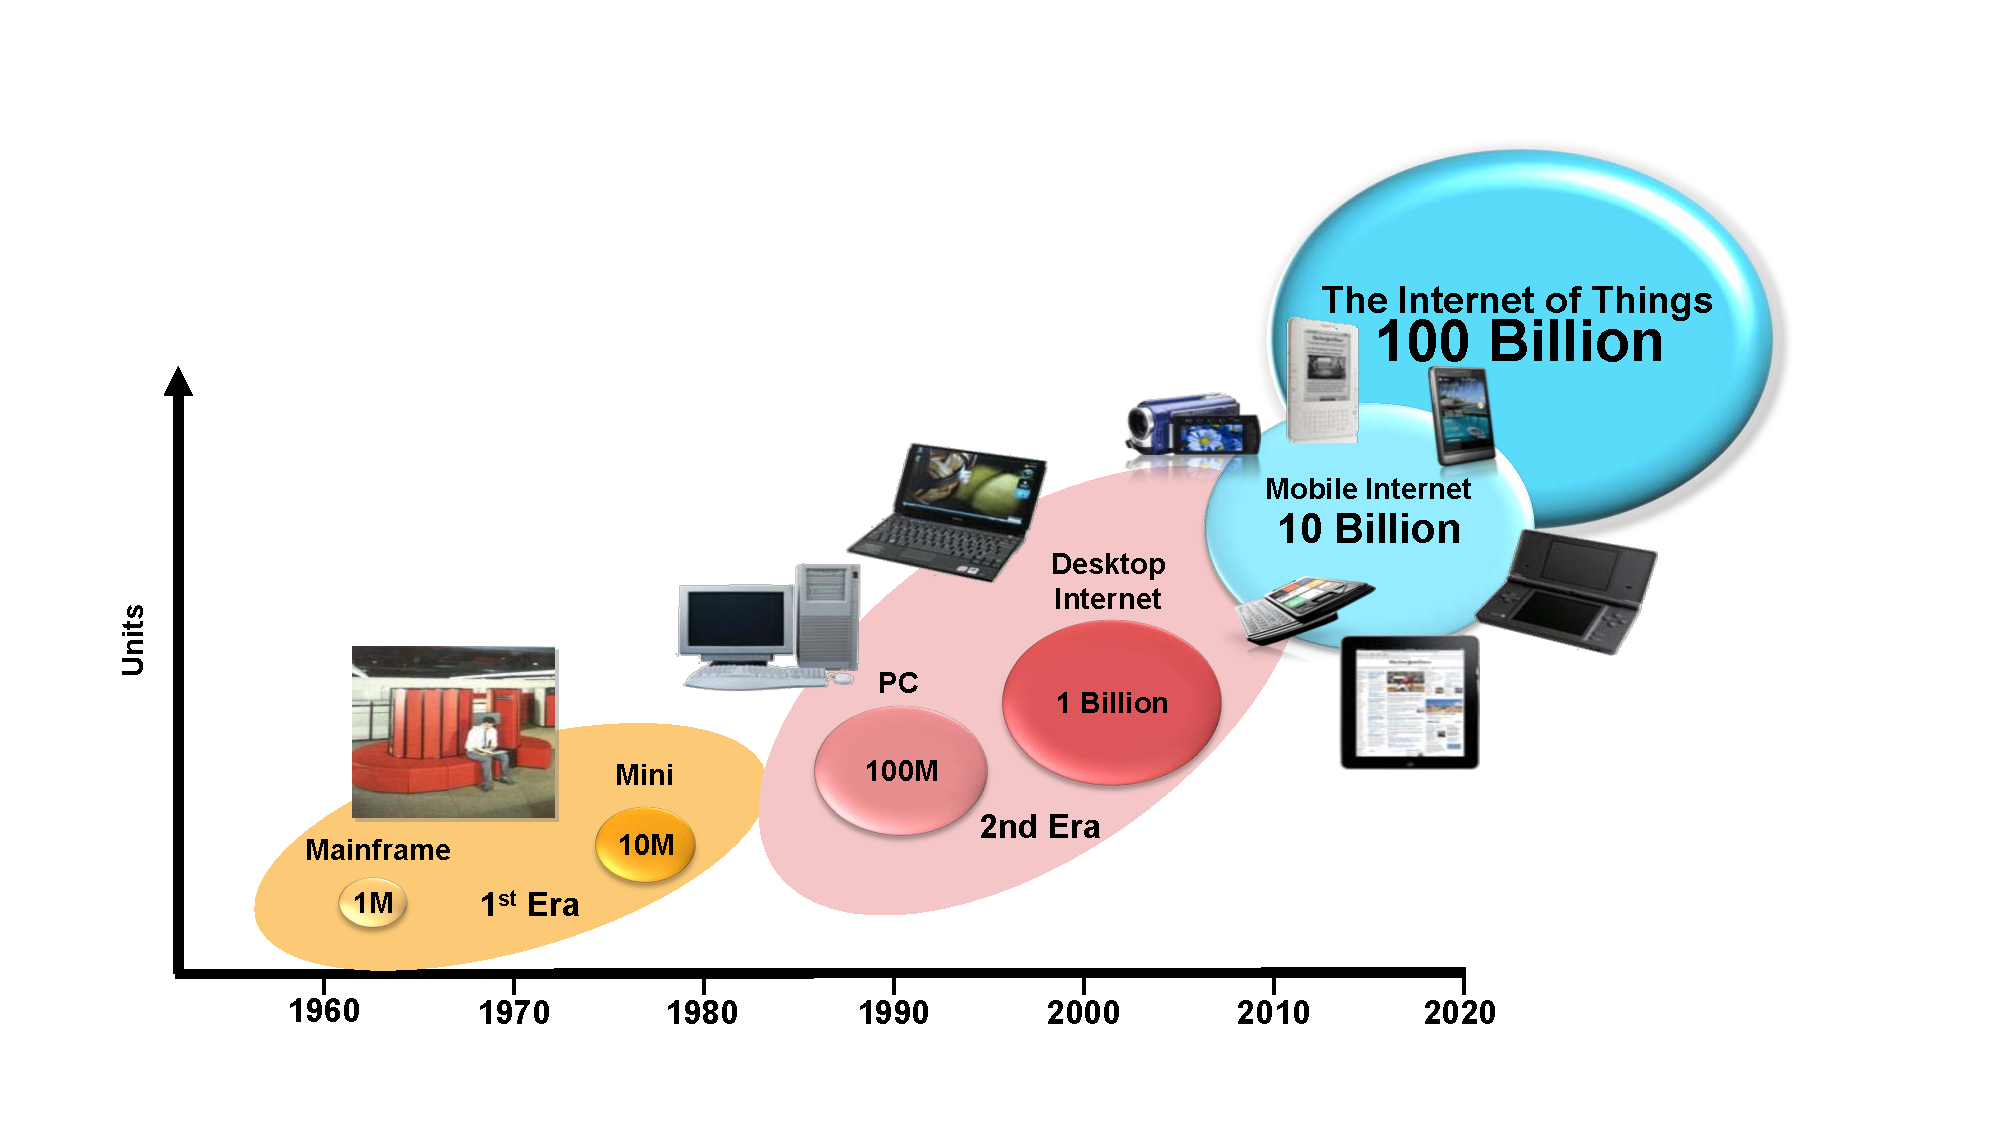
\includegraphics[width=\textwidth]{enc/imagens/CompEras.pdf}
    Fonte:~\textcite{ARM2013}
\end{figure}


As bases teóricas e princípios da Engenharia de Computação remetem a computação, matemática, ciência e engenharia resolvendo problemas técnicos por meio do \textit{design} de dispositivos computacionais, \textit{software}, redes e processos \cite{CE2016}. Essas bases teóricas sustentam a atuação profissional em diferentes áreas, como melhor descrito na Seção~\ref{sec:atuacao}.


\section{Campos de Atuação Profissional}~\label{sec:atuacao}

%Na atuação profissional, as atribuições profissionais relacionadas ao bacharel em Engenharia de Computação segue as atribuições profissionais constantes de leis, decretos leis, resolução específica ou instrumento normativo existentes, podendo ser citadas as seguintes atuações:

%O Anexo II da Resolução do CONFEA n° 1010, de 22 de agosto de 2005, intitulado como Sistematização dos Campos de Atuação Profissional, estabelece as atribuições profissionais do bacharel em Engenharia de Computação no Brasil. Os itens citados na Resolução são:
\begin{itemize}
    \item Informação: Sistemas, Métodos e Processos da Informação e da Computação.
    \item Sistemas Operacionais: Organização de Computadores. Compiladores.
    Paradigma de Programação. Algoritmos e Estrutura de Dados. Softwares Aplicados à Tecnologia.
    \item Pesquisa Operacional: Modelagem, Análise e Simulação de Sistemas. Expressão Gráfica Computacional.
    \item \textit{Hardware}: Redes Lógicas. Técnicas Digitais. Informática Industrial.
    Instalações, Equipamentos, Componentes e Dispositivos de Mecânica Fina, Elétricos, Eletrônicos, Magnéticos e Ópticos da Engenharia de Computação.
\end{itemize}


\section{Objetivos do Curso}
\label{sec:objetivos}

O objetivo geral do Curso de Engenharia de Computação é a preparação de profissionais para serem capazes de receber e atender demandas e responsabilidades em um campo de atuação amplo que inclui:
\begin{itemize}
    \item Atuação em empresas de tecnologia e \textit{start ups} que desenvolvem sistemas computacionais (hardware e/ou software), tais como: Apple, Samsung, Amazon, Foxconn, Alphabet Inc., Microsoft, Huawei, etc.
    % parece estranho listar essas empresas aqui: por que essas e não outras? e se alguma 'pisar na bola'? vale a pena manter esta lista aqui?  (helio)
    \item A prática da Engenharia de Computação no mercado em diferentes verticais de atuação tais como: Agronegócio, Saúde, Aviação, Energia, Mineração, Petróleo, Finanças, Educação, Varejo, Serviços, Telecomunicações e Governo entre outras;
    \item Carreiras acadêmicas em Engenharia de Computação, através de uma sólida preparação para pós-graduação e posteriormente atuação no ensino, pesquisa e extensão.
\end{itemize}

O profissional formado em Engenharia de Computação (EC) deverá possuir a competência (conhecimento, habilidade e atitude) para atuar em diferentes áreas, incluindo Engenharia Elétrica, Engenharia de Automação, Engenharia de Produção, Tecnologia da Informação, Ciências da Computação e Física, entre outras áreas, de forma que habilita o egresso a ter competências para entender, mapear, propor e implementar soluções integradoras que atendam os requisitos do problema através de execução de projeto de engenharia que atenda a demanda.
% parece estranho indicar que o profissional pode atuar em áreas de formação de outros cursos. (helio)

Essas competências são adquiridas por meio de núcleos de formação que contemplam aspectos técnicos e também humanísticos, componentes curriculares que tratam as ações práticas, de saber fazer, conjuntamente com os aspectos teóricos e corpo docente qualificado e atuante nas esferas do ensino, da pesquisa e da extensão, criando oportunidades de aprendizado em sintonia com as demandas do mercado e da sociedade.


\section{Justificativa da Criação do Curso na UFSCar e sua Evolução Institucional}


O curso de Engenharia de Computação da UFSCar, implantado em 1992, e contemplando trinta vagas, foi aprovado através do Parecer n° 275/92, de 15 de abril de 1992, do Conselho de Ensino e Pesquisa e da Resolução n° 133/92, de 07 de maio de 1992, do Conselho Universitário da Universidade Federal de São Carlos, sendo reconhecido pela Portaria MEC n° 919, de 21 de agosto de 1998, cuja renovação do reconhecimento ocorreu através da Portaria SERES/MEC n° 286, de 21 de dezembro de 2012 (D.O.U. 27/12/2012).

O curso foi criado para atender às necessidades do mercado de trabalho que exigia profissionais com formação plena em engenharia e formação profissional em computação, pautado pelas diretrizes da Resolução CEF n° 48/76.

Nessa perspectiva, o curso almejava formar profissionais que projetassem sistemas computacionais, ou adaptasse os existentes, a partir do levantamento das necessidades de uma organização, dos estudos relativos à viabilidade técnica e custos do projeto, bem como realizaria o acompanhamento de todas as etapas da produção industrial. Esse profissional também seria formado para participar de projetos em indústrias, elaborando e utilizando novas técnicas de programação, modelagem e simulação de sistemas, que garantissem o emprego eficiente dos recursos computacionais.

% A Matriz Curricular de 1992 encontra-se no Anexo~\ref{cha:Matriz1992}, na qual as disciplinas são separadas por semestre e número de créditos. A distribuição da carga horária do curso também pode ser observada no Anexo~\ref{cha:Matriz1992} e a quantidade de créditos e as horas das disciplinas, divididas em seus tipos de Formação e referentes à Legislação Específica também.

Em 1996, ainda durante o processo de implantação do Curso de Bacharelado em Engenharia de Computação foi realizada a primeira autoavaliação com a participação de 4 (quatro) turmas de discentes, docentes e técnico-administrativos. Esse processo de autoavaliação vinculou-se ao Programa de Avaliação Institucional das Universidades Brasileiras (PAIUB), com financiamento da Secretaria de Ensino Superior (SESu/MEC), tendo o curso sido analisado considerando o perfil do profissional formado, os currículos e programas, as condições de funcionamento e os desempenhos docente e discente. Um resumo dos principais resultados da autoavaliação do PAIUB encontra-se em~\textcite{CPA}.

Em 1998, foi realizada a avaliação externa no período de reconhecimento do Curso pela equipe de avaliadores externos e nomeados pelo Ministério da Educação e Cultura (MEC). Os resultados dessa avaliação externa foram considerados positivos e um resumo dos indicadores da avaliação podem ser encontrados em~\textcite{CPA}. Nessa ocasião, a partir dos dados relativos à autoavaliação e avaliação externa, a carga horária total foi alterada de 252 (3.780 horas) para 250 créditos (3.750 horas), bem como algumas alterações na matriz curricular foram implementadas.

%De modo geral, essas alterações foram pautadas pelas mudanças identificadas no mercado de trabalho, ou seja, se fazia necessário propiciar o desenvolvimento de competências para a resolução de problemas que surgiram com o processo de implantação da Internet no Brasil. %A nova matriz elaborada em 1999 encontra-se no Anexo~\ref{cha:Matriz1999}.

A primeira reformulação curricular foi implementada em 2006 e pautou-se pela ampliação de conteúdos do núcleo básico, reorganização das práticas de laboratório para subsidiar a solução de problemas baseados na integração dos projetos multidisciplinares então existentes. A inclusão de disciplinas optativas vinculadas às linhas de pesquisa do corpo docente do Departamento de Computação seja no Programa de Mestrado em Ciência da Computação, como no Programa de Mestrado em Biotecnologia propiciou uma formação geral sólida para que o discente pudesse: (i) atuar nos mais diversos ramos de atividades da Engenharia de Computação; (ii) buscar consolidar a realização de seus interesses individuais; e (iii) estivesse preparado para enfrentar os desafios tecnológicos. Outro aspecto da avaliação vinculado à reformulação se refere ao Exame Nacional de Desempenho de Estudantes (ENADE) para os cursos de Computação, realizado pela primeira vez em 2005, quando entre estudantes com as melhores notas, figuraram os do curso de Bacharelado em Engenharia de Computação da UFSCar, campus São Carlos.

Em 2015 foi instituída uma comissão para a reformulação do projeto pedagógico, motivada pelos avanços tecnológicos, novos aspectos sócios econômicos existentes e novas avaliações do curso realizadas pela Comissão Própria de Avaliação (CPA) da UFSCar, criada a partir da publicação da Lei n° 10.861 de 14 de abril de 2004, que instituiu o Sistema Nacional de Avaliação da Educação Superior (SINAES). Este projeto pedagógico foi aprovado em 2018 (aprovado pelo Conselho de Curso da EC em sua 45ª reunião ordinária de 12/07/2018 e pelo Conselho do Departamento de Computação em sua 3ª reunião extraordinária de 13/07/2018) e implementado para os ingressos de 2019, de forma que a primeira turma concluirá o curso no final de 2023. As alterações no curso se caracterizaram por um melhor balanceamento da carga horária das disciplinas, com ênfase maior em disciplinas de \textit{hardware}. De forma geral, o curso como um todo teve sua carga horária total reduzida para 3.660~horas e teve como alterações relevantes a inserção de disciplinas eletivas e o cumprimento obrigatório de atividades complementares, com destaque a projetos integradores com caráter extensionista. Tais modificações permitiram que o curso assumisse uma identidade própria, tanto frente a outros cursos de Engenharia de Computação quanto aos demais cursos a área de Computação. 

% TODO: pensar se deixa simples ou mais completo o texto...
%Em 2019 foram instituídas as novas Diretrizes Curriculares Nacionais de Ensino (DCNs), as quais trazem, entre outros aspectos, a ênfase no desenvolvimento de competências técnicas e sócio emocionais dos estudantes ao longo da sua trajetória de formação. 

Desde 2001, com a aprovação do Plano Nacional de Educação, as DCNs se estabeleceram como padrão de orientação acerca da elaboração dos currículos e projetos pedagógicos pelas IES. Daí em um movimento contínuo, houve a mudança de visão de formação do egresso com o paradigma da formação de suas competências. Em 2019, a Câmara de Educação Superior do Conselho Nacional de Educação (CES/CNE) através da Resolução nº 02/2019, estabelecem as novas DCNs onde são definidos os princípios, os fundamentos, as condições e as finalidades baseadas nas competências a serem adquiridas pelos egressos.  

As novas DCNs trazem, entre outros aspectos, a ênfase no desenvolvimento de competências técnicas e sócio emocionais dos estudantes ao longo da sua trajetória de formação, buscando criar um ambiente propício para o desenvolvimento do pensamento criativo, com sólida base teórica, da capacidade de inovação e de empreendedorismo dos graduandos em engenharia.

Ainda nesse movimento das novas DCNs, estabeleceu-se, através da resolução Resolução Número 7, de 18 de Dezembro de 2018, as “Diretrizes para a Extensão na Educação Superior Brasileira”, a qual define os princípios, os fundamentos e os procedimentos que devem ser observados no planejamento nas políticas, na gestão e na avaliação das  instituições de educação superior de todos os sistemas de ensino do país em relação a extensão nos cursos de graduação.

Neste contexto, este novo PPC do curso de Bacharelado em Engenharia de Computação (EC) busca se adequar às novas DCNs e a curricularização da extensão atendendo às referidas diretrizes segundo o perfil do profissional a ser formado pela UFSCar (UFSCar, 2008) e a incorporação das Resoluções instituídas pela Câmara de Educação Superior do Conselho Nacional de Educação (CES/CNE).  % TODO: Rever este texto frente à incorporação de extensão.

% acho que falta também uma ligação desta informação com o conteúdo desta seção. (helio)